% !TeX document-id = {ff202395-b098-4bc3-9327-f6d40065422a}
%!TEX TXS-program:compile = txs:///xelatex/[--shell-escape]
%!TEX encoding = UTF-8 Unicode
\documentclass{lsbook}

\tcbuselibrary{listings}

\title{一个中文书籍的\LaTeX{}模板}
\DedicatedTo{需要一个书籍模板的人}
\subtitle{这里可以放一个副标题}
\author{张三}% 默认值
\BookSeries{计算机应用技术丛书}% 可取消
\BookIntroduction{这个图书模板是在群主网站上的一个封面模板的基础上改写而成的,设定了一些图书出版要素,设计了封面、扉页及版权页和封底的样式,修改了chapter的样式,并提供了几个选项可切换色彩风格,其余则维持book基本文档类的设定。\par 图书模板部分代码的完成得到了林莲枝大神的帮助,在此表示感谢。由于作者水平有限,模板代码编写不恰当之处还请用户提出批评和指正。\par 感谢造字工坊提供了刻宋、郎宋和黄金时代三种非商业可免费下载使用的字体。\par 感谢谷歌提供自由使用的思源宋体、思源黑体。\par 感谢文泉驿提供的开源的文泉驿等宽微米黑字体。}
\Publisher{\LaTeX Studio 出版社} %默认值
\Designer{张三丰}
\Editor{张三丰}
\edition{2}% 可取消
\Price{26.5}
\isbn{978-80-7340-097-2}

% 自己所有的设置都放到settings.tex里面

\usepackage{amsfonts,amssymb}
\usepackage{amsmath}
\DeclareMathOperator{\argmin}{argmin}

\usepackage[mathbf=sym,math-style=TeX]{unicode-math}

\usepackage[math-style=TeX]{unicode-math}


%\setmathfont{texgyrepagella-math.otf}[math-style=TeX]
%\usepackage{bm}

\usepackage{extarrows}

\usepackage[c1]{optidef}


% hyperlink
\usepackage[colorlinks=true,hidelinks]{hyperref}


\def\equationautorefname~#1\null{公式(#1)\null}%
\def\footnoteautorefname{脚注}%
\def\itemautorefname~#1\null{第#1项\null}%
\def\figureautorefname{图}%
\def\tableautorefname{表}%
\def\partautorefname~#1\null{第#1部分\null}%
\def\appendixautorefname{附录}%
\def\chapterautorefname~#1\null{第#1章\null}%
\def\sectionautorefname~#1\null{第#1节\null}%
\def\subsectionautorefname~#1\null{第#1小节\null}%
\def\subsubsectionautorefname~#1\null{第#1小小节\null}%
\def\paragraphautorefname~#1\null{第#1段\null}%
\def\subparagraphautorefname~#1\null{第#1小段\null}%
\def\theoremautorefname{定理}%
\def\pageautorefname~#1\null{第~#1~页\null}%

\RequirePackage[nameinlink]{cleveref}      % 'nameinlink' option emulates look of \autoref
\crefname{cvcounter}{Program List}{Program Lists} 

\crefrangeformat{equation}{公式~(#3#1#4) 至~(#5#2#6)}
\crefmultiformat{equation}{公式~(#2#1#3)}{ 和~(#2#1#3)}{, (#2#1#3)}{ 和~(#2#1#3)}

%\crefrangemultiformat{equation}{公式~(#2#1#3)}{, (#2#1#3)}{, (#2#1#3)}{和~(#2#1#3)}

\crefname{equation}{式}{公式}

\definecolor{mygreen}{rgb}{0,0.6,0}
\definecolor{mygray}{rgb}{0.5,0.5,0.5}
\definecolor{mymauve}{rgb}{0.58,0,0.82}

\xeCJKsetup {
	CheckSingle = true,
	AutoFallBack = true,
	AutoFakeBold = false,
	AutoFakeSlant = false,
	CJKecglue = {~},
	PunctStyle = kaiming,
	KaiMingPunct+ = {:;},
}


\begin{document}
\maketitle
\makeflypage
\frontmatter
\tableofcontents

\mainmatter
\chapter{模板使用说明}
首先我们简要说明一下目前已经开发出来的模板功能,包括字体选择和颜色选择。
\section{颜色选择}
目前颜色选择共三种,\texttt{green},\texttt{orange}和\texttt{violet},默认为\texttt{green}。你也可以自己设置 \texttt{cvprimary}, \texttt{cvsecondary} 以及 \texttt{cvtext},定制你自己喜欢的色盘。


\begin{tcblisting}{listing only,applelight,title={自己来设定颜色吧!},
  listing options={basicstyle=\ttfamily,columns=fullflexible,
  language={[LaTeX]TeX},moretexcs={colorlet,definecolor,PassOptionsToPackage}}
}
% 如果想要用 xcolor 宏包已定义的颜色,记得要在 \documentclass 之前
% 传递相应的 xcolor 选项。
\PassOptionsToPackage{dvipsnames}{xcolor}
\documentclass{lsbook}
% cvprimary 为封面、标题盒子最外围的颜色
\colorlet{cvprimary}{SkyBlue}
% cvsecondary 为封面、标题盒子主要填充的颜色
\colorlet{cvsecondary}{RoyalBlue}
% cvtext 为封面、标题盒子里文字的颜色,也可以自己给出
% 特定的色值。
\definecolor{cvtext}{HTML}{EEEEFF}
\end{tcblisting}


\section{字体选择}
目前字体选择共两种,\texttt{customfont}和\texttt{systemfont},默认为\texttt{systemfont}。
若要使用\texttt{customfont},需要安装相应的字体。
若要使用\texttt{systemfont},则模板直接调用系统内部字体。

\section{几个可有可无的 tcolorbox 设置}

现有 \texttt{appledark}, \texttt{applelight}, \texttt{win10dark}, \texttt{win10light} 四个选项。
如果是供荧幕阅读的还好;如果是要打印出来的,除非您就是打印店的老板,不然还是不要多用 \texttt{*dark} 选项。

\begin{tcolorbox}[appledark,title={世界你好!}]
天气好吗?吃饱了吗?
\end{tcolorbox}

\begin{tcolorbox}[applelight,title={世界你好!}]
天气好吗?吃饱了吗?
\end{tcolorbox}
\subsection{Ubuntu Terminal}
\begin{GitExampla}{TensorFlow@xubuntu:$\sim$}
TensorFlow@xubuntu:~$
---------- TRAINING -------------
Epoch: 004/020 cost: 1.41867 train_accuray:0.63000 test_accuray:0.62820
Epoch: 008/020 cost: 0.98922 train_accuray:0.71000 test_accuray:0.72040
Epoch: 012/020 cost: 0.81536 train_accuray:0.70000 test_accuray:0.76270
Epoch: 016/020 cost: 0.71605 train_accuray:0.83000 test_accuray:0.78570
Epoch: 020/020 cost: 0.65017 train_accuray:0.82000 test_accuray:0.80130
\end{GitExampla}
\mybox{灰色主题的盒子}
\begin{tcolorbox}[win10dark,title={世界你好!}]
天气好吗?吃饱了吗?
\end{tcolorbox}

\begin{tcolorbox}[win10light,title={世界你好!}]
天气好吗?吃饱了吗?
\end{tcolorbox}

\chapter{代码盒子}
\begin{langCVOne}{SIFT算法}
# -*- coding: utf-8 -*-
"""
Created on Wed Jan 22 19:22:10 2014

@author: duan
"""

import cv2
import numpy as np

img = cv2.imread('home.jpg')
gray= cv2.cvtColor(img,cv2.COLOR_BGR2GRAY)

sift = cv2.SIFT()
kp = sift.detect(gray,None)

img=cv2.drawKeypoints(gray,kp)

cv2.imwrite('sift_keypoints.jpg',img)
\end{langCVOne}
\begin{langCVOne}[matlab][m:2]{Matlab求解}
b1 = [-6;0];
a1 = [-3 -2;1 0];
d1 = [0;5/2];
format rat;
alpha1 = b1\(a1*d1) % 右乘a1
\end{langCVOne}
\begin{langPyOne}{Haar cascading detection in OpenCV}
# -*- coding: utf-8 -*-
"""
Created on Thu Jan 30 11:06:23 2014

@author: duan
"""

import numpy as np
import cv2

face_cascade = cv2.CascadeClassifier('haarcascade_frontalface_default.xml')
eye_cascade = cv2.CascadeClassifier('haarcascade_eye.xml')

img = cv2.imread('sachin.jpg')
gray = cv2.cvtColor(img, cv2.COLOR_BGR2GRAY)

# Detects objects of different sizes in the input image.
# The detected objects are returned as a list of rectangles.
# cv2.CascadeClassifier.detectMultiScale(image, scaleFactor, minNeighbors, flags, minSize, maxSize)
# scaleFactor – Parameter specifying how much the image size is reduced at each image
# scale.
# minNeighbors – Parameter specifying how many neighbors each candidate rectangle should
# have to retain it.
# minSize – Minimum possible object size. Objects smaller than that are ignored.
# maxSize – Maximum possible object size. Objects larger than that are ignored.
faces = face_cascade.detectMultiScale(gray, 1.3, 5)
for (x,y,w,h) in faces:
    img = cv2.rectangle(img,(x,y),(x+w,y+h),(255,0,0),2)
    roi_gray = gray[y:y+h, x:x+w]
    roi_color = img[y:y+h, x:x+w]
    eyes = eye_cascade.detectMultiScale(roi_gray)
    for (ex,ey,ew,eh) in eyes:
        cv2.rectangle(roi_color,(ex,ey),(ex+ew,ey+eh),(0,255,0),2)
cv2.imshow('img',img)
cv2.waitKey(0)
cv2.destroyAllWindows()
\end{langPyOne}
\begin{langPyTwo}[python]{Single GPU computation time: 0:00:11.833497\\Multi GPU computation time: 0:00:07.085913}{Multi-GPU Basics}
import numpy as np
import tensorflow as tf
import datetime

#Processing Units logs
log_device_placement = True

#num of multiplications to perform
n = 10

# Example: compute A^n + B^n on 2 GPUs

# Create random large matrix
A = np.random.rand(1e4, 1e4).astype('float32')
B = np.random.rand(1e4, 1e4).astype('float32')

# Creates a graph to store results
c1 = []
c2 = []

# Define matrix power
def matpow(M, n):
    if n < 1: #Abstract cases where n < 1
        return M
    else:
        return tf.matmul(M, matpow(M, n-1))

# Single GPU computing

with tf.device('/gpu:0'):
    a = tf.constant(A)
    b = tf.constant(B)
#compute A^n and B^n and store results in c1
c1.append(matpow(a, n))
c1.append(matpow(b, n))

with tf.device('/cpu:0'):
    sum = tf.add_n(c1) #Addition of all elements in c1, i.e. A^n + B^n

t1_1 = datetime.datetime.now()
with tf.Session(config=tf.ConfigProto(log_device_placement=log_device_placement)) as sess:
# Runs the op.
    sess.run(sum)
    t2_1 = datetime.datetime.now()

# Multi GPU computing
# GPU:0 computes A^n
with tf.device('/gpu:0'):
#compute A^n and store result in c2
    a = tf.constant(A)
    c2.append(matpow(a, n))

#GPU:1 computes B^n
with tf.device('/gpu:1'):
#compute B^n and store result in c2
b = tf.constant(B)
c2.append(matpow(b, n))

with tf.device('/cpu:0'):
    sum = tf.add_n(c2) #Addition of all elements in c2, i.e. A^n + B^n

t1_2 = datetime.datetime.now()
    with tf.Session(config=tf.ConfigProto(log_device_placement=log_device_placement)) as sess:
# Runs the op.
sess.run(sum)
t2_2 = datetime.datetime.now()

print "Single GPU computation time: " + str(t2_1-t1_1)
print "Multi GPU computation time: " + str(t2_2-t1_2)
\end{langPyTwo}

\begin{GitExample}{Output Data}{TensorFlow@xubuntu:$\sim$}
TensorFlow@xubuntu:~$ python3 test.py
Extracting data/train-images-idx3-ubyte.gz
Extracting data/train-labels-idx1-ubyte.gz
Extracting data/t10k-images-idx3-ubyte.gz
Extracting data/t10k-labels-idx1-ubyte.gz
train shape: (55000, 784) (55000, 10)
test  shape: (10000, 784) (10000, 10)
----------MNIST loaded----------------
NeuralNetwork Ready!
2018-08-02 00:11:15.818190: I tensorflow/core/platform/cpu_feature_guard.cc:137] Your CPU supports instructions that this TensorFlow binary was not compiled to use: SSE4.1 SSE4.2 AVX AVX2 FMA
2018-08-02 00:11:16.044897: I tensorflow/core/common_runtime/gpu/gpu_device.cc:1030] Found device 0 with properties:
name: GeForce GTX 1080 Ti major: 6 minor: 1 memoryClockRate(GHz): 1.582
pciBusID: 0000:0a:00.0
totalMemory: 10.92GiB freeMemory: 3.04GiB
2018-08-02 00:11:16.044948: I tensorflow/core/common_runtime/gpu/gpu_device.cc:1120] Creating TensorFlow device (/device:GPU:0) -> (device: 0, name: GeForce GTX 1080 Ti, pci bus id: 0000:0a:00.0, compute capability: 6.1)
---------- TRAINING -------------
Epoch: 004/020 cost: 1.41867 train_accuray:0.63000 test_accuray:0.62820
Epoch: 008/020 cost: 0.98922 train_accuray:0.71000 test_accuray:0.72040
Epoch: 012/020 cost: 0.81536 train_accuray:0.70000 test_accuray:0.76270
Epoch: 016/020 cost: 0.71605 train_accuray:0.83000 test_accuray:0.78570
Epoch: 020/020 cost: 0.65017 train_accuray:0.82000 test_accuray:0.80130

Extracting data/train-images-idx3-ubyte.gz
Extracting data/train-labels-idx1-ubyte.gz
Extracting data/t10k-images-idx3-ubyte.gz
Extracting data/t10k-labels-idx1-ubyte.gz
train shape: (55000, 784) (55000, 10)
test  shape: (10000, 784) (10000, 10)
----------MNIST loaded----------------
NeuralNetwork Ready!
2018-08-02 00:11:15.818190: I tensorflow/core/platform/cpu_feature_guard.cc:137] Your CPU supports instructions that this TensorFlow binary was not compiled to use: SSE4.1 SSE4.2 AVX AVX2 FMA
2018-08-02 00:11:16.044897: I tensorflow/core/common_runtime/gpu/gpu_device.cc:1030] Found device 0 with properties:
name: GeForce GTX 1080 Ti major: 6 minor: 1 memoryClockRate(GHz): 1.582
pciBusID: 0000:0a:00.0
totalMemory: 10.92GiB freeMemory: 3.04GiB
2018-08-02 00:11:16.044948: I tensorflow/core/common_runtime/gpu/gpu_device.cc:1120] Creating TensorFlow device (/device:GPU:0) -> (device: 0, name: GeForce GTX 1080 Ti, pci bus id: 0000:0a:00.0, compute capability: 6.1)
\end{GitExample}
\section{settings.sty的一些设置和宏包的使用}
\begin{langCVOne}[matlab][m:2]{Matlab求解}
b1 = [-6;0];
a1 = [-3 -2;1 0];
d1 = [0;5/2];
format rat;
alpha1 = b1\(a1*d1) % 右乘a1
\end{langCVOne}

得$\hat{a}_k=\dfrac{6}{5}$

$\succeq\succ\prec\preceq$$xyz\textsl{x}\text{x}$

\begin{align*}
\nabla_xL(x,\nu) = 2x + A^T\nu = 0,
\end{align*}
\subsection{线性规划问题}
\mybox{考虑标准形式的线性规划问题}
\begin{mini}[2]
	{}{c^Tx}
	{\label{eq:Ex1}}{}
	\addConstraint{Ax = b}
	\addConstraint{x \succeq 0}
\end{mini}

\begin{align*}
b^T &= \begin{bmatrix}
b_1 & b_2 & \cdots & b_n
\end{bmatrix}\\
x^T &= \begin{bmatrix}
x_1 & x_2 & \cdots & x_n
\end{bmatrix}\\
b^T\nu &= \nu^Tb
\end{align*}

如果我们猜测$x$的值为$\hat{x}$,也就是隐含地猜测$v$的值为$y-A\hat{x}$。假设$v$(在$\|\cdot\|$度量下)越小越可信,那么对于$x$的最有可信的猜测是
\begin{align}
\hat{x} = \argmin_z	\|Az - y\|
\end{align}

考虑子空间$\symcal{A} = \symcal{R}(A)\subseteq\symbf{R}^m$和一个点$b\in\symbf{R}^m$。点$b$向子空间$\symcal{A}$的\textsf{投影}是$\symcal{A}$中在$\|\cdot\|$下最靠近$b$的点,也就是说,它是下列问题的任意最优解
\begin{mini}[2]
	{}{\|u-b\|}
	{\label{eq:Ex1}}{}
	\addConstraint{u\in \symcal{A}.}
\end{mini}
将$\symcal{R}(A)$中的元素参数化为$u=Ax$,我们可以看出求解范数逼近问题(6.1)等价于计算$b$向$\symcal{A}$的投影。

Newton方法是求解无约束优化问题的有效算法,干净优化问题的一个特例就是经常遇到的最小二乘问题
\begin{mini}[2]
	{}{\|Ax-b\|_2^2 = x^T(A^TA)x-2(A^Tb)^Tx+b^Tb}
	{\label{eq:Ex2}}{}
\end{mini}
其最优性条件
\[
A^TAx^\ast = A^Tb
\]
被称为最小二乘问题的\textsf{正规方程}
\mbox{无约束几何规划}
作为第二个盒子,我们考虑凸的无线事几何规划问题
\begin{mini}[2]
	{}{f(x) = \log \left(\sum_{i=1}^{m}\exp(a^T_ix+b_i)\right)}
	{\label{eq:Ex2}}{}
\end{mini}
其最优性条件为
\[
\nabla f(x^\ast) = \frac{1}{\sum\limits_{j=1}^m\exp(a^T_jx^\ast + b_j)}\sum_{i=1}^{m}\exp(a^T_ix^\ast+b_i)a_i=0.
\]
一般情况下该方程组没有解析解,因此我们必须采用迭代算法。由于$\symbf{dom}f=\symbf{R}^n$,斜体点都可以用作初始点$x^{(0)}$。

\begin{align}\label{eq:3}
f(y) \leqslant f(x) + \nabla f(x)^T(y-x) + \frac{m}{2}\|y-x\|^2
\end{align}
对任意固定的$x$,\cref{eq:3}的右边是$y$的二次凸函数。令其关于$y$的层数等于零,即
\begin{align}\label{eq:4}
\frac{\partial\bigl[f(x) + \nabla f(x)^T(y-x) + \frac{m}{2}\|y-x\|_2^2\bigr]}{\partial y} &= 0\\
0 + \nabla f(x) + m(y-x) &=0\label{eq:5}
\end{align}
其中$y>x$,可以得到该二次函数的最优解$\tilde{y}=x-(1/m)\nabla f(x)$。

二次型函数极点
\[\left(-\frac{b}{2a},\frac{4ac-b^2}{4a}\right)\]
\mybox{unicode-math的一些说明}
这里使用的数学宏包是unicode-math,所以一些命令与amsmath里面有些不同

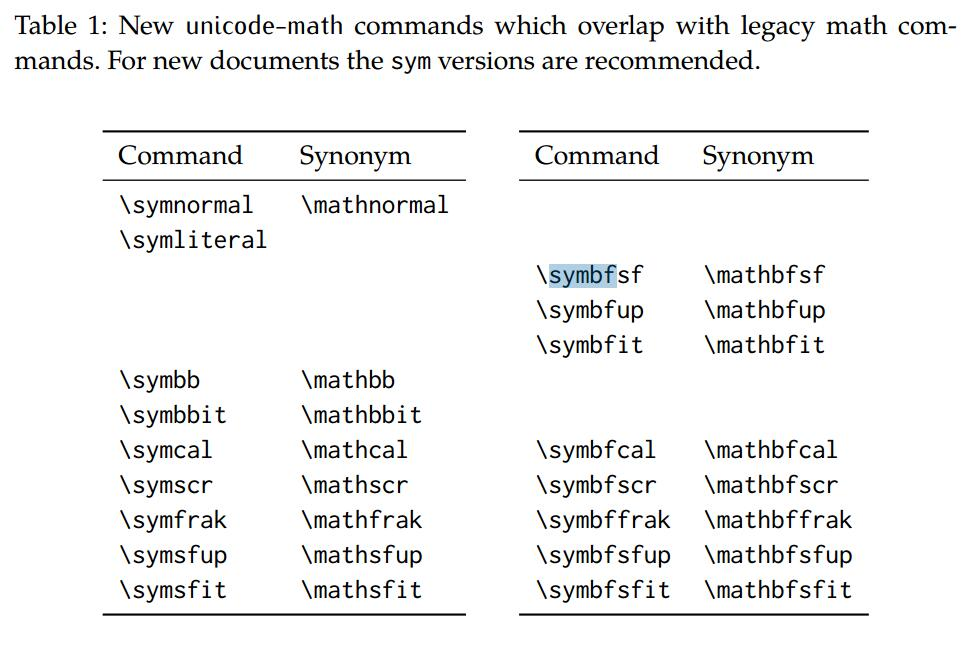
\includegraphics[width=0.7\linewidth]{unimath}

\makebackcover
\end{document}
